\section{Reštiev}
Najprej si poglejmo, kako se obnašajo energije z različnimi algoritmi,
ali se ohranjajo ali ne. Poglejmo si že implementirane
algortime v \verb|scipy.ivp_solve()|.
\begin{figure}[h]
    \centering
    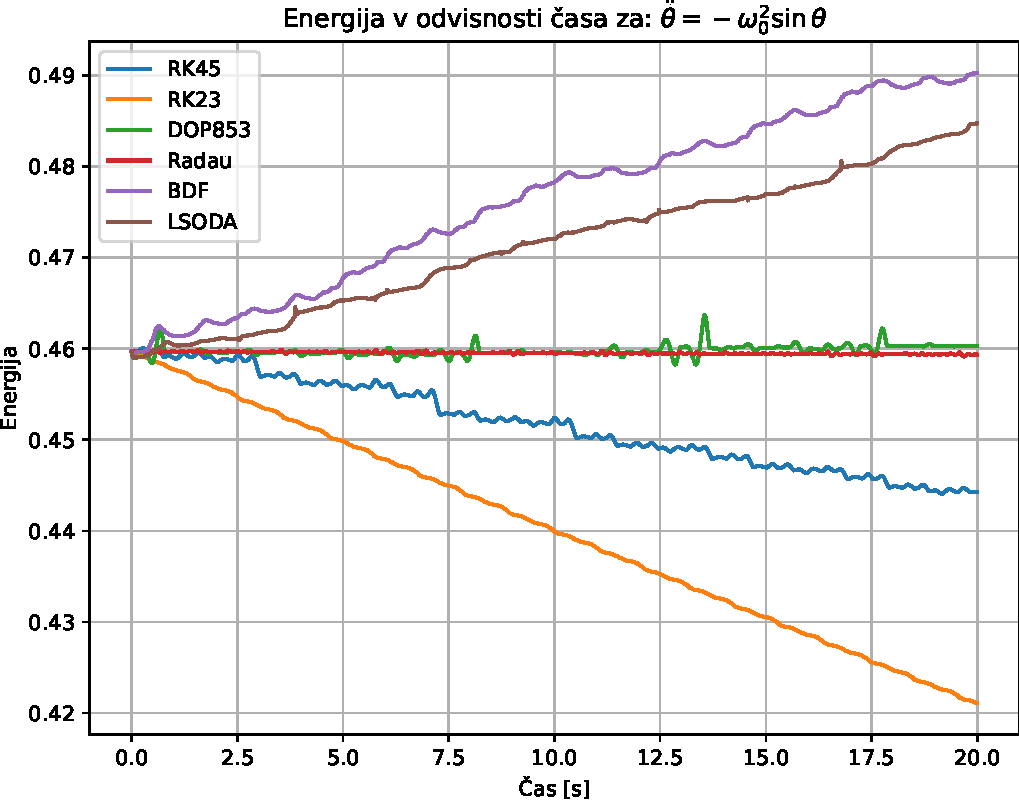
\includegraphics[width=12cm]{pdfs/energije.pdf}
    \caption{Ohranjanje energije pri različnih algoritmih}
\end{figure}
Od tu vidimo, da je najbolj uporabna metoda \verb|Radau|, ki jo bomo v nadaljevanju vedno uporabljali.
Poglejmo si še časovno odvisnost algoritmov, ki ohranjajo energijo.
\begin{figure}[h]
    \centering
    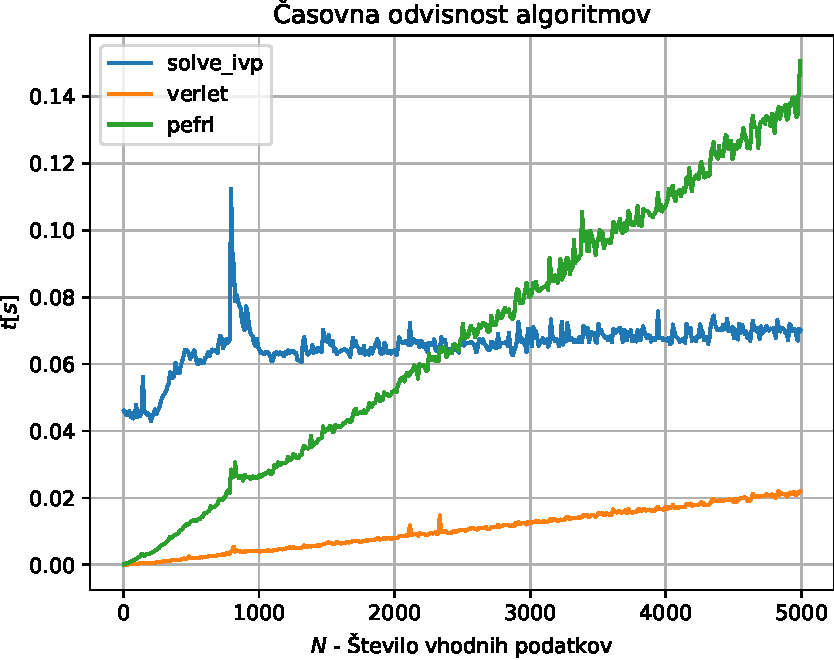
\includegraphics[width=8cm]{pdfs/time.pdf}
    \hfill
    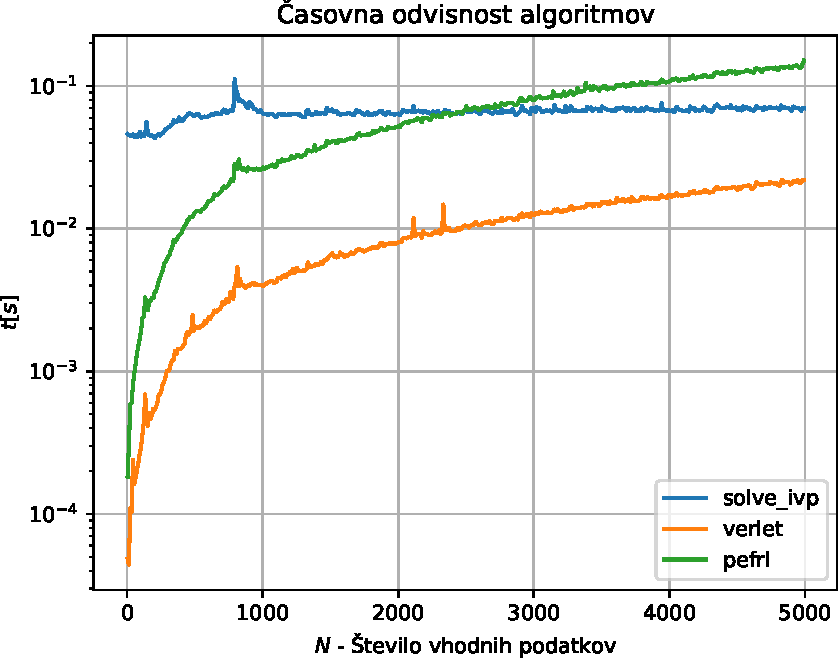
\includegraphics[width=8cm]{pdfs/timelog.pdf}
    
    \caption{Časovna odvisnost različnih algoritmov}
\end{figure}
\newpage 
Poglejmo si še trajektorijo nihala.
\begin{figure}[h]
    \centering
    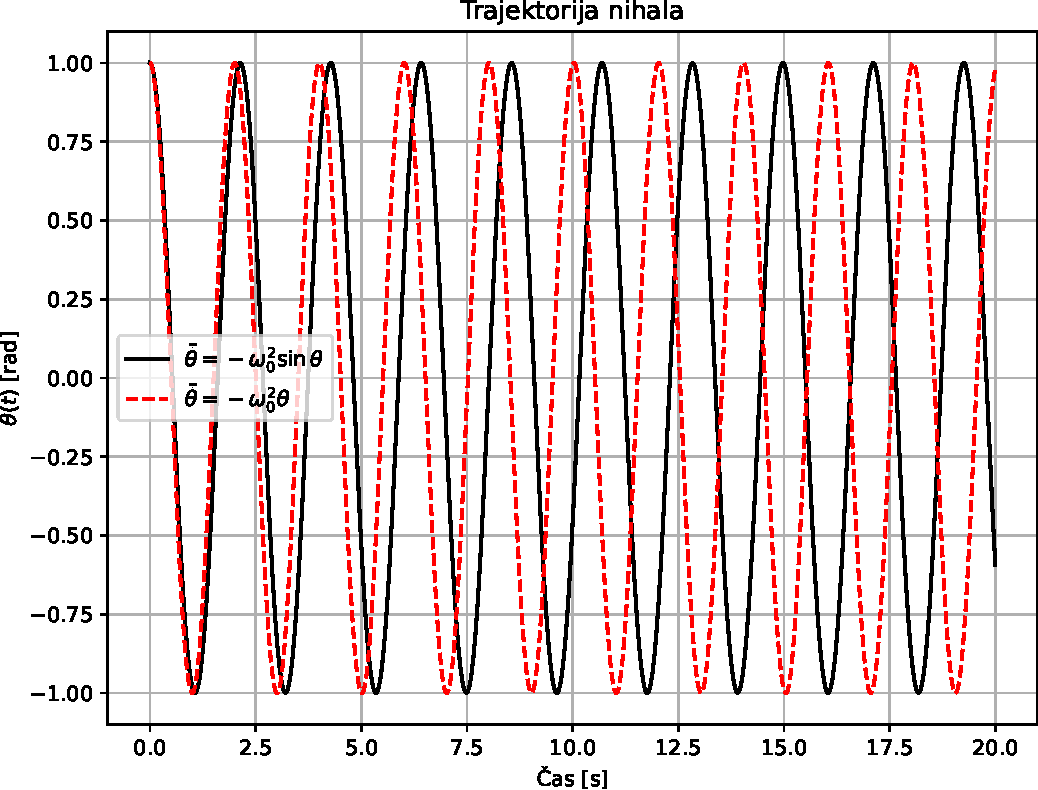
\includegraphics[width=12cm]{pdfs/trajektorija.pdf}
    \caption{Trajektorija pravega nihala in matematičnega nihala}
\end{figure}
Poglejmo si še kako vpliva začetna lega na frekvenco, izračunano: $\omega = \frac{2\pi}{t_0}$, kjer je $t_0$
obhodni čas.
\begin{figure}[h]
    \centering
    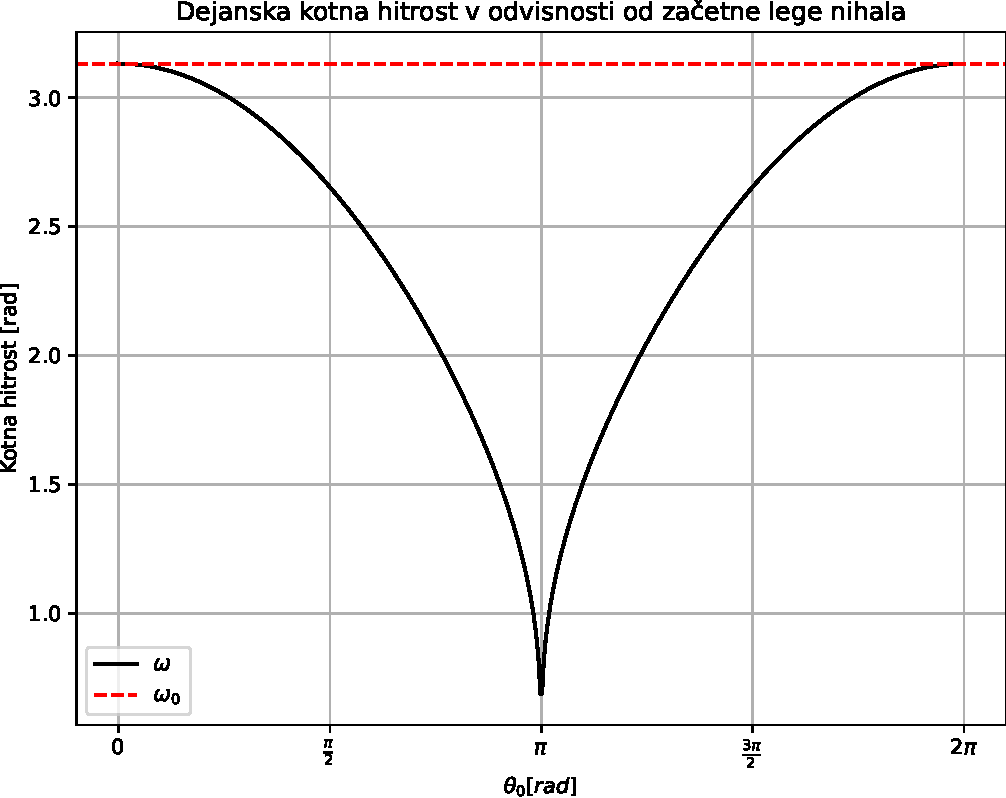
\includegraphics[width=10cm]{pdfs/w(theta).pdf}
    \caption{Odvisnost frekvence matematičnega in točnega nihala od začetne lege}
\end{figure}
\newpage
Polgejmo si še fazni diagram:
\begin{figure}[h]
    \centering
    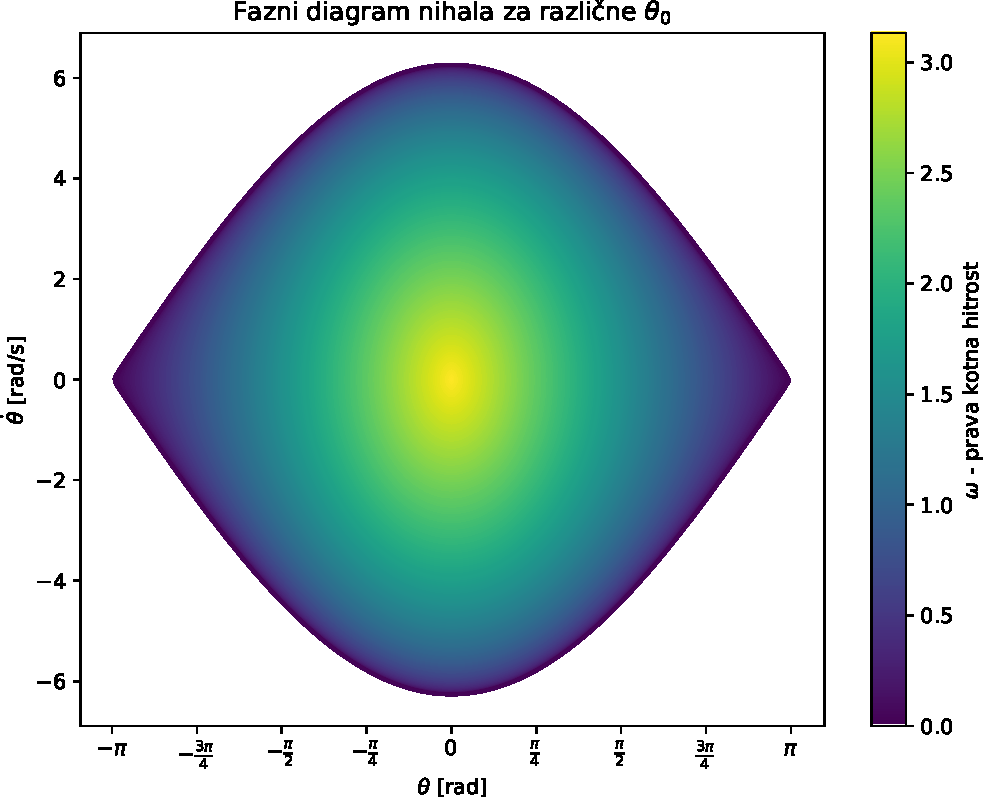
\includegraphics[width=\textwidth]{pdfs/fazni_dig.pdf}
    \caption{Fazni diagram $\dot{\theta}(\theta)$}
\end{figure}
